%% $Id: scene-backend-management.tex,v 1.4 2002/07/10 14:10:48 ayla Exp $
%%
%% Documentation to explain how the scene graph and OpenGL backend is
%% set up and run in FreeWRL.

\documentclass[12pt,letterpaper]{article}

\usepackage{freewrl}
\customheadings

\begin{document}

    The OpenGL libraries do the actual rendering work in the FreeWRL
    browser.
    Setting up the backend is done through FreeWRL's scene model
    \texttt{VRML::Scene}.
    The result of the initialization steps described in the next section
    is the scene graph for the VRML input files and the associated backend
    to OpenGL.

    \section{VRML statements}

	%%\subsection{PROTO}

    %% better explain the browser class and the event loop!

    \section{FreeWRL Initialization}

	\subsection{Scene Graph}

	The scene graph is a tree constructed by parsing a VRML input file and
	building a tree of VRML nodes starting from the parent (root) node.
	%%If the parent node is a PROTO\ldots
	An example of a scene graph corresponding to the following VRML code
	is represented as a tree is shown in Figure~\ref{fig:sg-tree}.

	New node types are defined using either the PROTO or EXTERNPROTO
	(new node type defined in external file) keywords.
	These nodes are handled differently than the node types defined in the
	VRML standard.
	A new PROTO definition must be broken down into a \uline{name},
	\uline{field types}, \uline{field kinds} (ie. EventIn, EventOut,
	ExposedField), default field values and a \uline{parent} node.
	See the VRML97 standard for a full description of node types and PROTO
	definitions~\cite{web3D:vrml97}.
	Inline nodes are treated as PROTOs for the purposes of building the
	backend to the OpenGL module.


	\begin{verbatim}
	    [pick a VRML example from the FreeWRL tests]
	\end{verbatim}

	\begin{figure}[!ht]
	    \centering
	    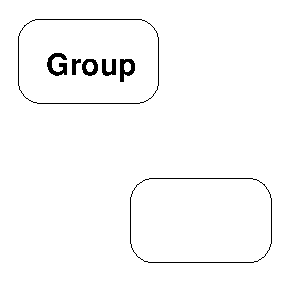
\epsfig{file=fig/sg-tree.eps}
	    \caption{}\label{fig:sg-tree}
	\end{figure}

	The parser (\texttt{VRML::Parser}) is responsible for parsing the text
	of a VRML input file and calling on the scene object to build the
	appropriate node representation.
	The browser (\texttt{VRML::Browser}) is responsible for calling the
	methods to construct the scene graph.

	%% lame - needs way more explaination!
	This is done either when a string containing the text of a VRML input
	file is loaded (\texttt{VRML::Browser::load\_string}) or when a world is
	replaced (\texttt{VRML::Browser::replaceWorld}).

	%% DEF nodes
	%% USE nodes
	%% IS statements

	The scene object prepares the newly construted scene graph and it's
	constituent nodes for rendering by calling
	\texttt{VRML::Scene::make_executable}.

	\subsection{Backend}

	During initialization, a series of function calls are made to
	build FreeWRL's backend to OpenGL.
	These function calls are summarized in Figure~\ref{fig:be-setup}.

	\begin{figure}[!ht]
	    \centering
	    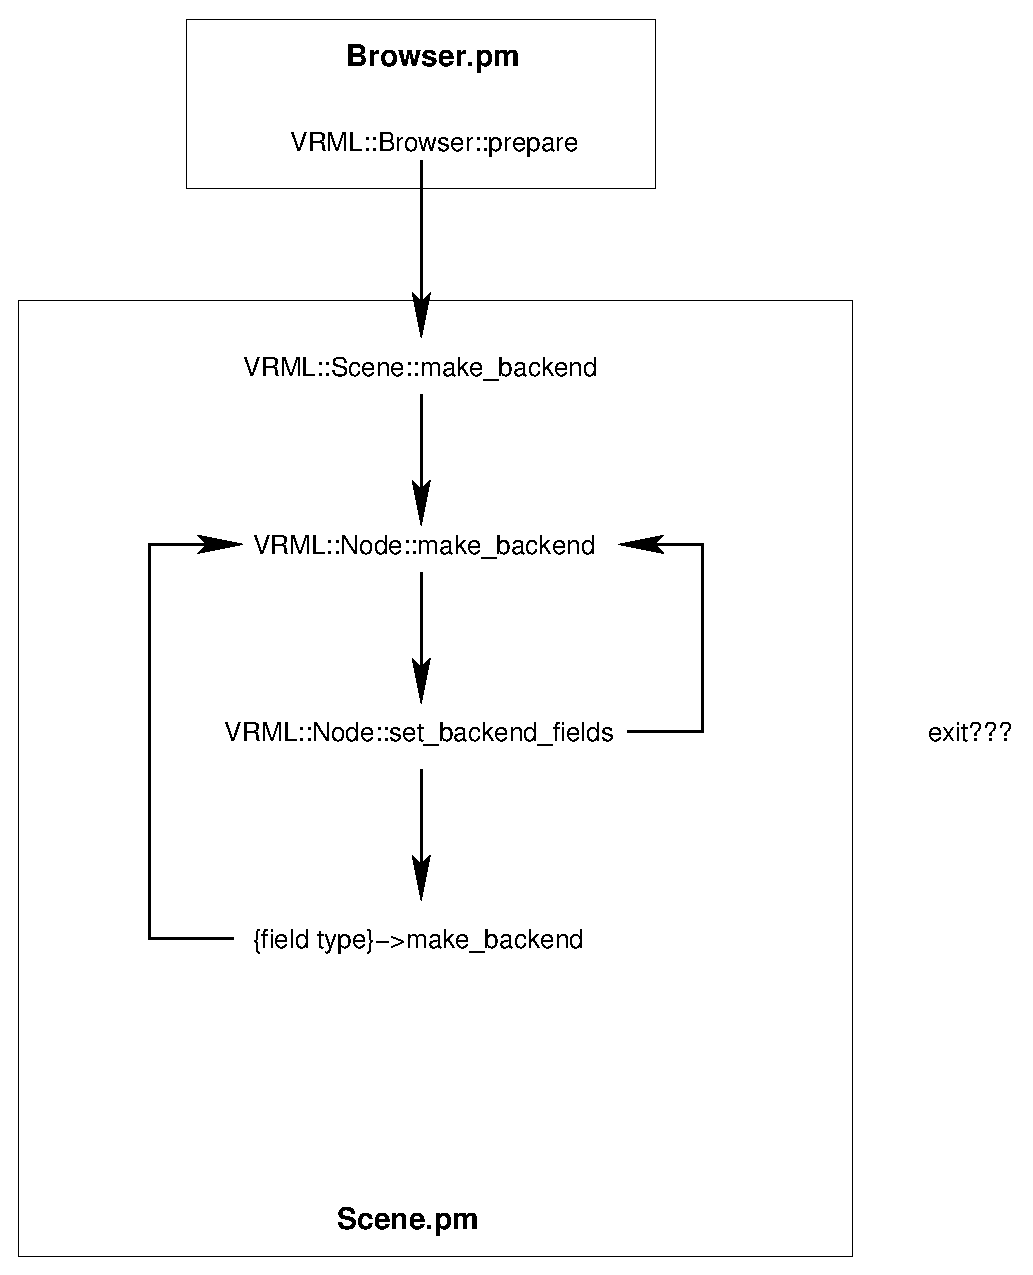
\epsfig{file=fig/be-setup.eps,width=12cm}
	    \caption{Function calls to set up the FreeWRL backend.}\label{fig:be-setup}
	\end{figure}

	The browser contains the backend structure, which is used in the event
	loop to update the scene displayed by FreeWRL.

	\bibliographystyle{plain}
	\bibliography{freewrl-cites}

\end{document}
